\section{Application 2: Posterior Sampling for Bayesian Optimization}
\label{sec:sampling_results}

The second application of CIQ we explore is GP posterior sampling in the context of Bayesian optimization \citep[e.g.][]{snoek2012practical}.
Bayesian optimization methods aim to find the maximum (or minimum) of a black-box function $g(\cdot)$
(e.g. $g(\cdot)$ is the validation error of a neural network as a function of hyperparameters).
A Gaussian process $f(\cdot)$ is typically used as a surrogate model, modelling the probabilistic beliefs about $g(\cdot)$ based on previous observations $\dset_N = (\bx_1, g(\bx_1)), \ldots, (\bx_N, g(\bx_N))$ (e.g. previous hyperparameter configurations).
At each iteration, we select a new point acquisition point $\bx_{N+1}$; we evaluate $g(\bx_{N+1})$; and then we update our posterior belief over $f$.

To select the new point $\bx_{N+1}$, we evaluate an {\bf acquisition function} at many possible candidate points $\mathcal{T} = \{ \bxtest_1, \ldots, \bxtest_T \}$.
Intuitively, an acquisition functions determines how useful it would be to evaluate $g(\bxtest_i)$.
Many acquisition functions require drawing samples from the current GP posterior $p(f(\bxtest_1), \ldots, f(\bxtest_T) \mid \dset)$.
One canonical example is {\bf Thompson Sampling} \cite{thompson1933likelihood}, which trades off exploitation of existing minima for exploration of new potential minima.
Thompson sampling simply chooses $\bx_N$ as the minimizer of a sample $f(\cdot)$ drawn from the posterior.
%
\[
  \bx^\text{(Thompson)}_{N+1} = \argmin_{\bx_i \in \mathcal{T}} f(\bx_i),
  \quad
  f(\cdot) \sim p(f(\cdot) \mid \dset_N).
\]
%
Let $\bmeantest \in \reals^{T}$ and $\Covtest \in \reals^{T \times T}$ be the posterior mean and covariance evaluated at $\bxtest_1$, $\ldots$, $\bxtest_T$.
For each iteration of Thompson sampling we draw a sample via
%
\begin{equation}
  \meantest + {\Covtest}^{\frac 1 2} \bepsilon,
  \quad
  \bepsilon \sim \normaldist{\bzero}{\bI}.
  \label{eqn:thompson_sample}
\end{equation}
%
In many Bayesian optimization, the candidate points $\bxtest_1$, $\ldots$, $\bxtest_T$ are uniformly sampled in the search space \cite{balandat2019botorch}.
Larger values of $T$ more densely cover the search space, which naturally should result in better acquisition points.
It is therefore beneficial to choose the largest value of $T$ that is computationally feasible.
Using Cholesky to compute \cref{eqn:thompson_sample} incurs a $\bigo{T^3}$ cost which severely limits the size of $T$.
On the other hand, CIQ is only $\bigo{T^2}$, can be preconditioned, and more readily utilizes GPU acceleration.
When used in the conjunction with kernel partitioning methods that will be described in the next chapter, the memory requirement of CIQ can also be reduced to $\bigo{N}$ (see \cref{sec:largeexact_method}).


\subsection{Results}

We perform Bayesian optimization on three high-dimensional black-box functions: a classical test function ({\bf Hartmann}, $D=6$) and two robotics simulations ({\bf Lunar Lander}, $D=12$; {\bf Rover}, $D=60$).
For each problem we use exact Gaussian processes (no approximations) as the surrogate model and Thompson sampling as the acquisition function.
Our goal is to determine whether CIQ-based sampling is beneficial by allowing us to scale to larger candidate set sizes.

\paragraph{Baselines.}
Here, we limit the baseline methods to exact sampling methods, and therefore do not consider stochastic approximations \cite{rahimi2008random} or methods that rely on inducing points \cite{wilson2020efficiently}.
Consequentially, we do not compare against LOVE-based sampling from \cref{chapter:love} as its can only be used in conjunction with the KISS-GP approximation.
It is worth noting that, with sufficient quadrature points and msMINRES iterations, we can reduce the error of CIQ to machine precision (see \cref{thm:ciq_convergence}); therefore it can be considered an exact sampling method like Cholesky.

\begin{figure}[t!]
  \centering
  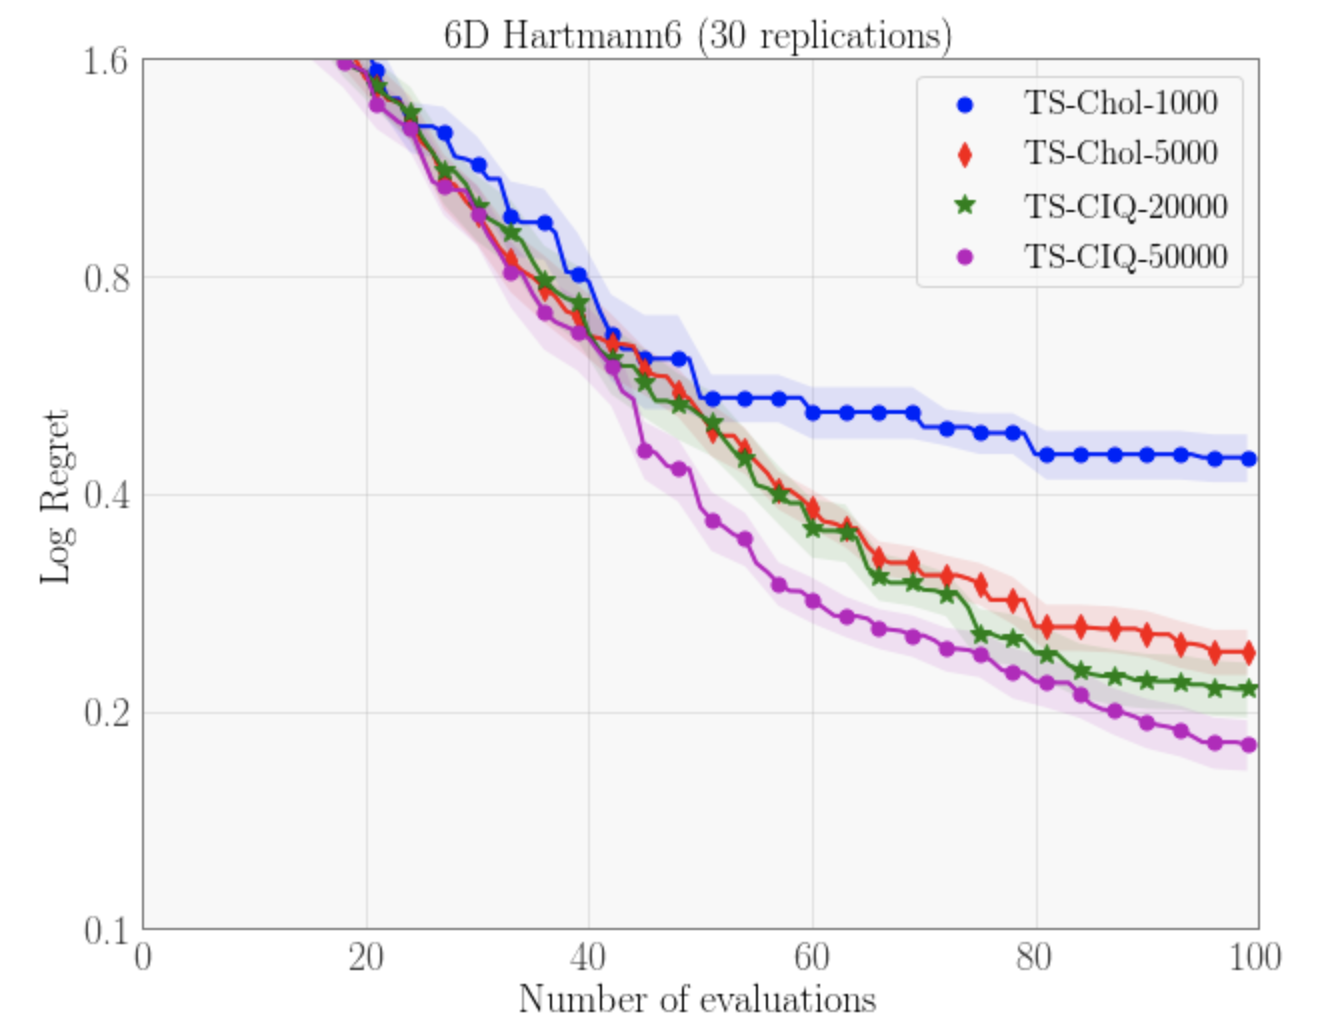
\includegraphics[width=0.72\linewidth]{figures/hartmann6.png}
  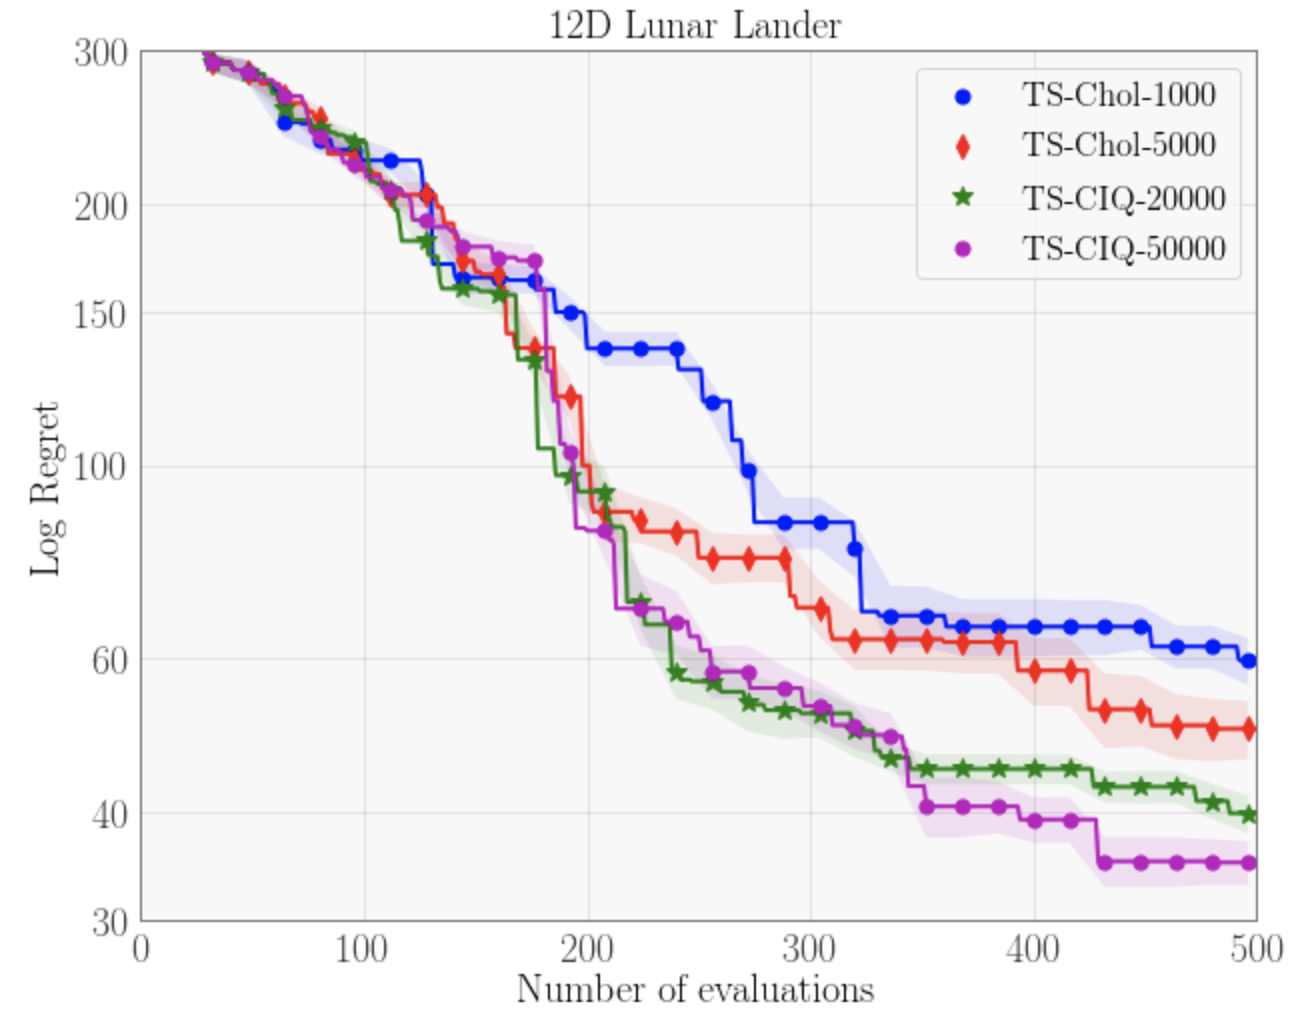
\includegraphics[width=0.7\linewidth]{figures/lunar_lander.png}
  \caption[
    A comparison of sampling methods for Bayesian optimzation (BayesOpt) via Thompson sampling.
    BayesOpt is applied to the Hartmann ($D=6$) and Lunar Lander ($D=12$) functions.
  ]{
    A comparison of sampling methods for Bayesian optimzation (BayesOpt) via Thompson sampling.
    BayesOpt is applied to the ({\bf top}) Hartmann ($D=6$) and ({\bf bottom}) Lunar Lander ($D=12$) functions.
    Methods: TS-Chol-$\langle T \rangle$ draws posterior samples with Cholesky at $T$ candidate points.
    TS-CIQ-$\langle T \rangle$ draws posterior samples with CIQ.
    Larger $T$ (number of candidate point) results in better optimization.
    CIQ enables scaling to $T\geq50,\!000$.
  }
  \label{fig:hartmann6_lunar}
\end{figure}

We measure the performance of Thompson sampling as a function of the candidate set size $T$.
We run Thompson sampling Bayesian optimization with $T=1,\!000$, $T=5,\!000$, $T=20,\!000$, and $T=50,\!000$.
We use Cholesky ({\bf TS-Chol}) for $T=1,\!000$ and $T=5,\!000$, and we use CIQ ({\bf TS-CIQ}) for $T=20,\!000$ and $T=50,\!000$.
Note that it would be very challenging and impractical to use Cholesky with $T\geq10,\!000$, both due to its quadratic memory and its cubic time complexity.

\paragraph{Experimental details.}
The Gaussian processes use RBF kernels and zero mean functions.
After each posterior update, we optimize the GP hyperparameters using 10 iterations of Adam with a learning rate of $0.1$.
The candidate sets are sampled uniformly at random from the input space.
As with the variational experiments, we use $Q = 15$ quadrature points for CIQ.
MINRES terminates when the $\bd_j$ vectors achieve a relative norm of $0.001$ or after $J=1,\!000$ iterations.
We use a partial pivoted Cholesky preconditioner of rank $R=20$ when drawing CIQ samples.

For the Hartmann and Lunar Lander problems we use standard Thompson sampling acquisition function.
At each iteration we draw 5 posterior samples and choose the acquisition point based on the minimum of all samples.
Due to the high-dimensionality of the Rover problem, we use Thompson sampling in conjunction with the trust-region BayesOpt method of \citet{eriksson2019scalable}.
We use separate candidate sets for each trust region, and similarly choose the next acquisition point based on 5 posterior samples.

\begin{figure}[t!]
  \centering
  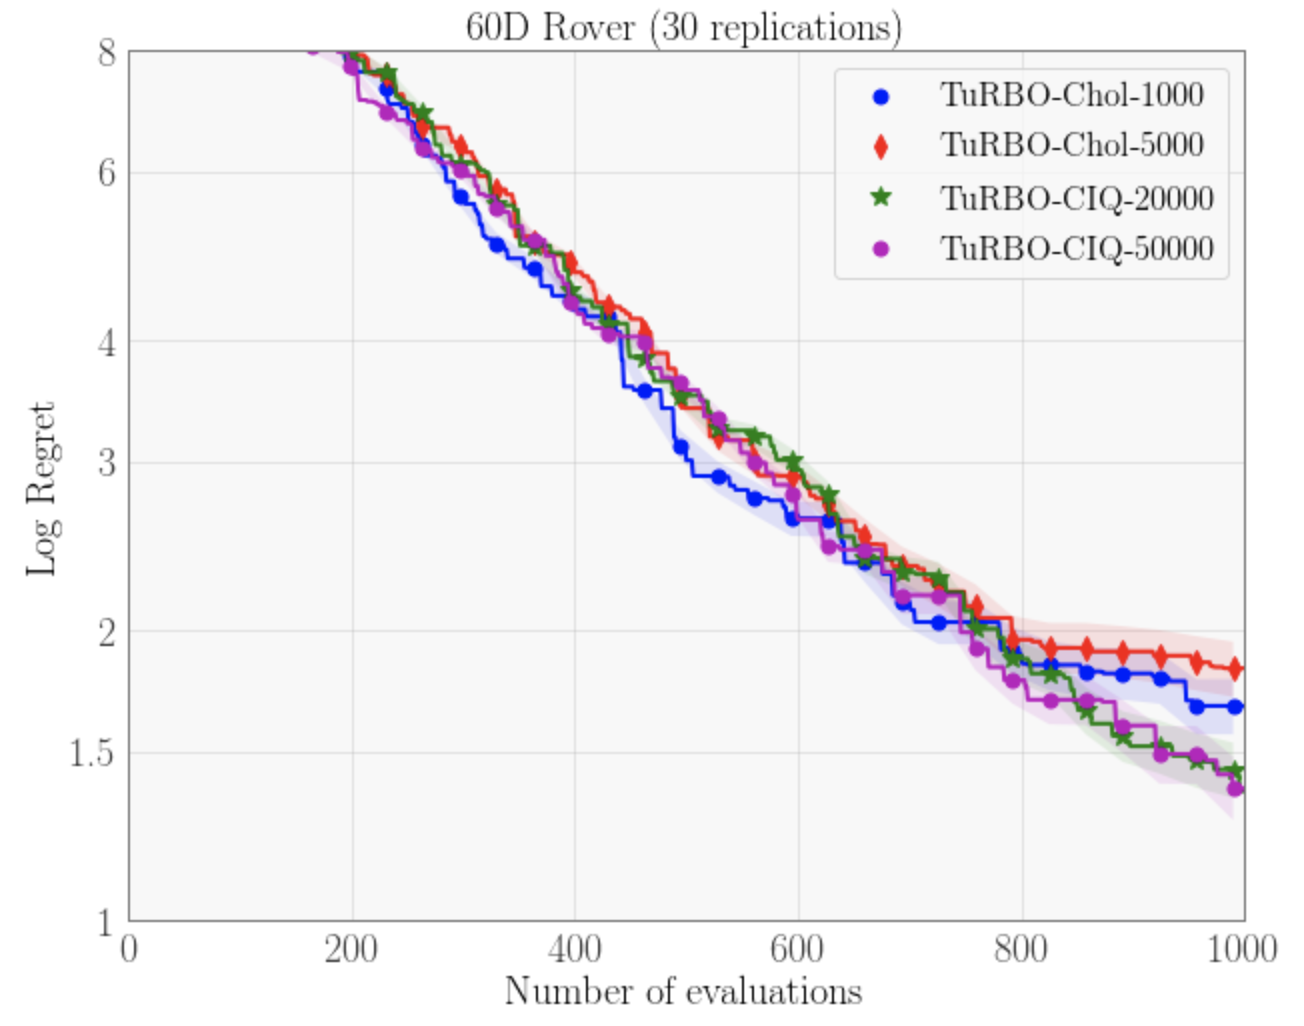
\includegraphics[width=0.7\linewidth]{figures/rover.png}
  \caption[
    A comparison of sampling methods for Bayesian optimzation (BayesOpt) via TuRBO \cite{eriksson2019scalable}.
    BayesOpt is applied to the Rover ($D=60$) function.
  ]{
    A comparison of sampling methods for Bayesian optimzation (BayesOpt) via TuRBO \cite{eriksson2019scalable}.
    BayesOpt is applied to the Rover ($D=60$) function.
    Larger $T$ (number of candidate point) results in better optimization.
    CIQ enables scaling to $T\geq50,\!000$, whereas Cholesky is limited to $T\leq5,\!000$
  }
  \label{fig:rover}
\end{figure}

\paragraph{Optimization performance.}
We plot the log regret of the Thompson sampling variants (Harmann and Lunar Lander in \cref{fig:hartmann6_lunar}, Rover in \cref{fig:rover}).
From these figures we can make several observations.
At early stages of optimization, the log regret is similar for all candidate set sizes.
However, in later stages of optimization we notice that larger candidate set sizes begin to have much lower regret.
By increasing $T=1,\!000$ to $T=50,\!000$, we cut the final log regret by substantial amounts on all problems.
On the Hartmann and Lunar Lander problems, we even see improved performance as we increase $T$ from $20,\!000$ to $50,\!000$.
It is therefore likely that even larger candidate set sizes could further improve optimization.

We re-iterate that $T=50,\!000$ is largely impractical with Cholesky sampling methods.
Large candidate sets have previously only been possible with approximate sampling methods.
CIQ enables us to scale to much larger values of $T$ without incurring additional bias or variance.
